\section{Q1. Diferenciar as Camadas 2 e 3 do modelo OSI e indicar os protocolos utilizados para endereçamento nestas camadas.}
\label{q1}

\subsection{Camada 2: Camada deEnlace de Dados}
A Camada de Enlace de Dados observa defeitos e corrige se necessário no pacote \cite{wikipedia2021enlace}. É nessa camada que é definida e topologia, e nela que há o funcionamento dos switches de camada 2.
Além disso, é nessa camada que é feito o controle de fluxo, para garantir que o emissor não envie dados rápido de mais para o receptor

Os protocolos mais utilizados são Ethernet e Wi\-fi, mas existem outros protocolos, como o token ring, FDDI (Fiber Distributed Data Interface), PPP (Point\-to\-Point Protocol), entre outros.

O protocolo de endereçamento desta camada é o próprio Ethernet, que define o formato do quadro (frame) com os campos de endereço MAC de origem e destino. Os endereços MAC são físicos e permanentes, inerentes a cada dispositivo (computador, celular, etc.), e ficam associados às portas dos switches por meio da tabela MAC, conforme a Figura \ref{fig:q1_mac_table}

\begin{figure}[H]
\centering
\caption{Tabela MAC de um switch}
\label{fig:q1_mac_table}
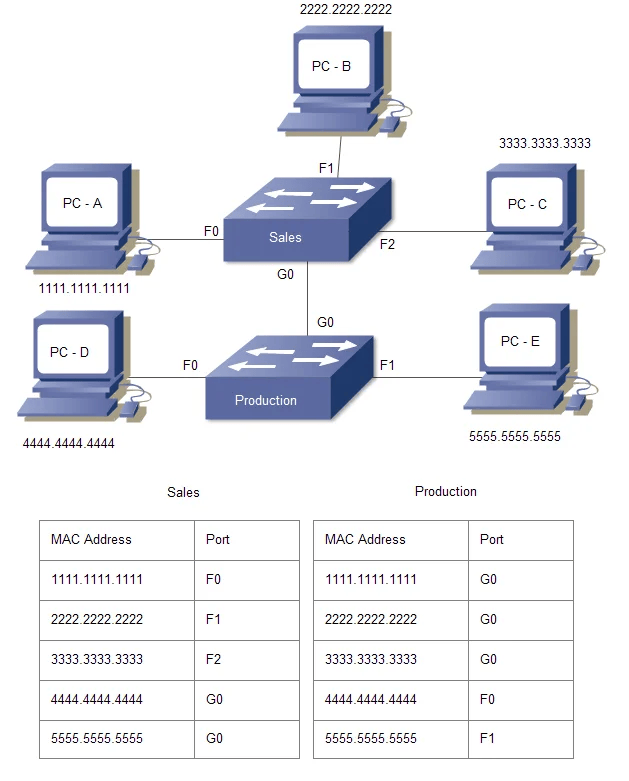
\includegraphics[width=0.8\textwidth]{imgs/tabelamac.png}
\legend{Fonte: \citeonline{CNN2026Lamix}, convertida para png pelo Autor}
\end{figure}

Esta tabela MAC é construída pelo próprio switch, por meio do processo de aprendizado de endereços: a cada frame recebido em uma porta, o switch registra o endereço MAC de origem e o associa a essa porta, montando a tabela de forma dinâmica conforme o tráfego passa pelo equipamento.

\subsection{Camada 3: Camada de Rede}
A camada de Rede \cite{wikipedia2024rede} define o caminho dos dados por meio dos algorítmos de roteamento, como o RIP, que conta o número saltos como métrica de eficácia (mas não leva em conta o tempo de atraso possível em cada salto), ou o OSPF (Open Shortest Path First), que tem como base o algorítmo de Dijkstra; é nessa camada que operam os switches de camada 3, que comunicam sub-redes.

Ela utiliza os protocolos IP e ICMP.
IP \cite{wikipedia2026ip}: Envia datagramas sem garantias, podendo chegar em parte desordenados, duplicados ou mesmo faltantes.
ICMP \cite{wikipedia2026icmp}: Composto principalmente de Echo Request e Echo Reply, ele é utilizado quando se quer verificar uma falha de comunicação entre dois dispositivos, com o comando PING.

Na camada de Rede também são definidos o IP e as subredes, por meio do mascaramento de IP, para conferir mais organizadas e seguras, isolando máquinas em subredes separadas.